\subsubsection{Backpropagation}\label{backpropagation}

En 1986, Rumelhart junto con otros investigadores publicaron “Learning representation by back-propagating errors” \cite{rumelhart}, un trabajo que volvió dar popularidad a las redes neuronales. El trabajo, basado en otros trabajos basados en diferenciación automáticas mostró experimentalmente como usando un nuevo algoritmo de aprendizaje se podría conseguir que una red neuronal se auto ajustará sus parámetros para así aprender una representación interna de la información que estaba procesando, un algoritmo conocido como \textit{backpropragation}.
\newline

Este algoritmo es adaptable a cualquier modelo y con él, dio por finalizado lo que históricamente se conoce como Invierno de la IA consiguiendo nuevas financiaciones y nuevos proyectos en el campo del \textit{Deep Learning}.
\newline

La predicción de un modelo se obtiene usando un algoritmo llamado \textit{feed-forward} como se ha explicado en la Sección \ref{feedforward}. Dicho valor debe ajustarse lo mejor posible al valor real. Para ello, se debe ir ajustando en un método iterativo las matrices $W$ en un proceso que se conoce como entrenamiento (ver Sección \ref{training}). En cada iteración del entrenamiento se irá ajustando las matrices $W$ haciendo uso primero de la función de coste, que mostrará la magnitud del error (ver Sección \ref{costfunction}), posteriormente ese error se irá propagando hacia atrás en el modelo para conocer la responsabilidad de cada neurona usando un algoritmo conocido como \textit{backpropagation} y finalmente, por cada neurona se calculará el vector gradiente $\nabla f$ que representa como ha afectado la neurona al resultado final y con ello se ajustarán sus distintos pesos $w$ y bias $b$(ver Sección \ref{minimizing-error}). 
\newline

El algoritmo de \textit{backpropagation} se puede representar gráficamente:

\begin{figure}[H]
    \centering
    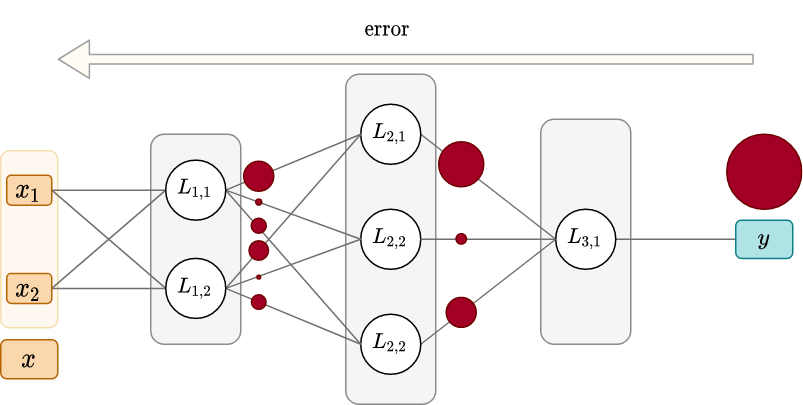
\includegraphics[width=14cm]{images/state-of-art/back-propagation/network_descent_gradient.png}
    \caption{Representación del algoritmo de backpropagation.}
    \label{fig:basic_network}
\end{figure}

En esta red se representa con círculos rojos el error de cada neurona. El error calculado por la función de coste es el error más grande que es el que está relacionado con la salida del modelo. A partir de ese punto, se retropropagará hacia atrás y se computará que parte del error pertenece a cada neurona hasta la primera capa. Por ejemplo, en la capa $L_2$, la principal neurona que tiene parámetros desajustados es $L_{2,1}$. A su vez, ese error principalmente tiene parte de la culpa debido a la neurona $L_{1,1}$. Por lo tanto, es lógico pensar que habría que ajustar neuronas como $L_{2,1}$ o $L_{1,1}$, sin embargo, dejar tal como están neuronas como $L_{1,2}$ o $L_{2,2}$.
\newline
 
A continuación, se define la red neuronal más simple que se puede construir con una sola neurona oculta y una neurona de salida.
\begin{figure}[H]
    \centering
    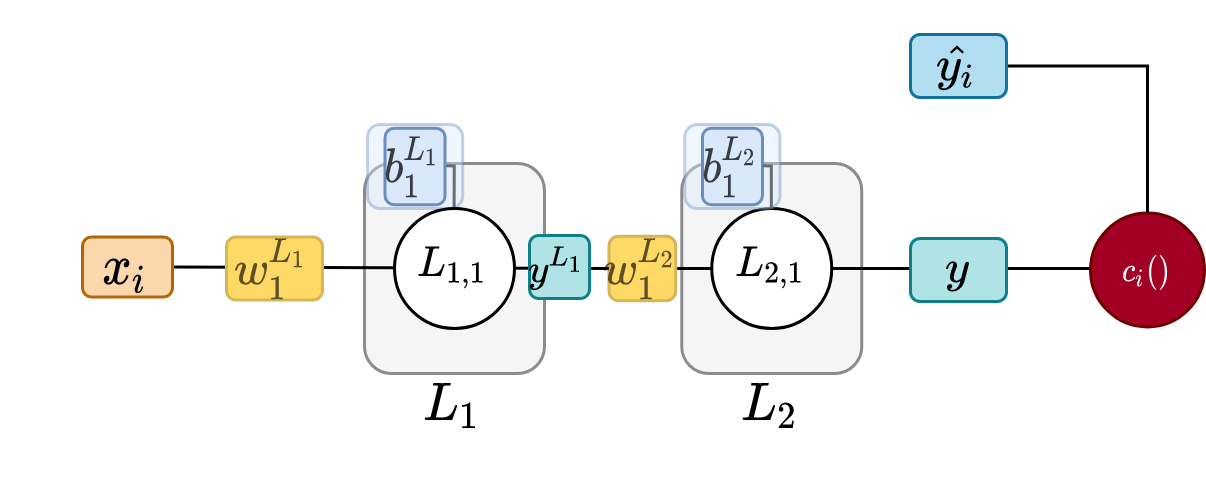
\includegraphics[width=12cm]{images/state-of-art/back-propagation/basic_network.png}
    \caption{Red neuronal básica.}
    \label{fig:basic_network}
\end{figure}

Para realizar el algoritmo de \textit{backpropagation}, primero se debe de computar la pérdida con la función $c_i$. Posteriormente, el algoritmo de \textit{backpropagation} "distribuirá" la pérdida del modelo a las capas anteriores (siempre se empieza por la última capa). Esta computación expresa cómo de importante son las matrices $W$ indicando cuánto impacto tiene en el modelo. Por ejemplo, si se cambia algún valor de $W_2$ de alguna forma, se podrá saber cómo afecta al resultado de la predicción del modelo. Matemáticamente:

\begin{equation}
\begin{split}
    \frac{\partial c}{\partial w^{L_2}} &= \frac{\partial c(a(z^{L_2}))}{\partial w^{L_2}} \\
    \frac{\partial c}{\partial b^{L_2}} &= \frac{\partial c(a(z^{L_2}))}{\partial b^{L_2}} 
    \label{eqn:backpropagationsimplenetworklayer2}
\end{split}
\end{equation}

El numerador es una composición de funciones, y es básicamente el cálculo del algoritmo \textit{feed-forward}(ver sección \ref{feedforward}). Para calcular la derivada parcial de una composición de funciones, hay que hacer uso de una herramienta de cálculo conocida como la regla de la cadena (\textit{chain rule}).
\newline

Un ejemplo para entender la \textit{chain rule} sería el siguiente. Se sabe que el Sol es $100$ veces más grande que la Tierra. A su vez, la Tierra es $4$ veces más grande que la Luna. Sabiendo esas dos relaciones, se puede saber cuánto es el Sol más grande que la Luna. Para ello simplemente multiplicamos $100 \times 4 = 400$. El sol por lo tanto es $400$ veces más grande que la Luna. Definiendo este problema con ecuaciones:

\begin{equation}
\begin{split}
    \frac{\partial T_{\text{Sol}}}{\partial T_{\text{Tierra}}} = 100
    \qquad
    \frac{\partial T_{\text{Tierra}}}{\partial T_{\text{Luna}}} = 4 \\
    \frac{\partial T_{\text{Sol}}}{\partial T_{\text{Luna}}} = \frac{\partial T_{\text{Sol}}}{\partial T_{\text{Tierra}}} \cdot \frac{\partial T_{\text{Tierra}}}{\partial T_{\text{Luna}}} = 400 \nonumber
\end{split}
\end{equation}

Se le llama la \textit{chain rule} porque se encadena en relación con el dato en común, en este caso $T_\text{Tierra}$ es la parte común que en un lado se encuentra en el denominador y en otro en el numerador. Por lo tanto, para derivar la composición de funciones vista en la Ecuación \ref{eqn:backpropagationsimplenetworklayer2}, simplemente hay que multiplicar cada una de las derivadas intermedias. Recordando las ecuaciones del algoritmo de \textit{feed-forward} y la composición de funciones para calcular el error del modelo para la red mostrada en la Figura \ref{fig:basic_network}:

\begin{equation}
\begin{split}
    z^{L_2} = W^{L_2} \cdot y^{L_1} + b^{L_2}
    \qquad
    c(a^{L_2}(z^{L_2}))
\end{split}
\end{equation}

Se calcula como se propaga el error de la capa $L_2$ a la capa $L_1$:

\begin{equation}
\begin{split}
     \frac{\partial c}{\partial w^{L_2}} &= \frac{\partial c}{\partial a^{L_2}} \cdot \frac{\partial a^{L_2}}{\partial z^{L_2}} \cdot \frac{\partial z^{L_2}}{\partial w^{L_2}} \\
     \frac{\partial c}{\partial b^{L_2}} &= \frac{\partial c}{\partial a^{L_2}} \cdot \frac{\partial a^{L_2}}{\partial z^{L_2}} \cdot \frac{\partial z^{L_2}}{\partial b^{L_2}}
\end{split}
 \label{eqn:backpropagationlayer2}
\end{equation}

Estas derivadas son fáciles de calcular y la explicación de cada derivada sería la siguiente:

\begin{itemize}
\item 1º derivada. Derivada de la función de activación respecto al coste:

\begin{equation}
    \frac{\partial c}{\partial a^{L_2}}
\end{equation}

Como varia el coste de la red (es la última capa) cuando se varía la salida de la función de activación de la red. En otras palabras, se calcula la derivada de la función de coste con respecto a la salida de la red neuronal. Es necesario, por tanto, saber la derivada de la función de coste usada.

\item 2º derivada. Derivada de la activación respecto a $z$:
\begin{equation}
    \frac{\partial a^{L_2}}{\partial z^{L_2}}
\end{equation}

Trata de reflejar como varía la salida de la neurona cuando se varía la suma ponderada de la neurona. La derivada que hay que usar es la derivada de la función de activación que se pueden ver en la sección \ref{activationfunction}. Derivada de la suma ponderada respecto a los valores de los pesos y bias.

\item 3º derivada: Derivada de $z$ respecto a los parámetros:
\begin{align*}
    \frac{\partial z^{L_2}}{\partial w^{L_2}} && \frac{\partial z^{L_2}}{\partial b^{L_2}}
\end{align*}

Indica como varía la suma ponderada $z$ con respecto a una variación de los parámetros. El parámetro $b$ es un valor independiente por lo que su derivada es una constante igual a $1$. Por otro lado, la derivada $\frac{\partial z^{L_2}}{\partial w^{L_2}}$ depende de la anterior capa.

\begin{align*}
    \frac{\partial z^{L_2}}{\partial w^{L_2}} = a^{L_1} && \frac{\partial z^{L_2}}{\partial b^{L_2}} = 1
\end{align*}

\end{itemize}

Partiendo de esta definición, se puede unir la 1º y 2º derivada en una sola:

\begin{equation}
     \frac{\partial c}{\partial a^{L_2}} \cdot \frac{\partial a^{L_2}}{\partial z^{L_2}} = \frac{\partial c}{\partial z^{L_2}}
\end{equation}

Esta derivada indica en qué grado se modifica el error cuando se produce un cambio en el error cuando se produce un pequeño cambio en la suma de las neuronas de la capa. Si el valor es grande es que ante un pequeño cambio en cualquiera de las neuronas de las capas en el valor $z$, se verá reflejado en el resultado del modelo. Por el contrario, si el valor es pequeño, un gran cambio en cualquiera de las neuronas en el valor de $z$ de no afectará al resultado final. En resumen, esta derivada muestra cómo afecta la capa (o alguna neurona en especial puesto que es un vector) en el resultado final y por lo tanto al error de la red y de esa forma el algoritmo del descenso del gradiente modificará los parámetros para poder obtener el mejor resultado posible. A esta derivada también se le conoce como el error imputado a la capa y se representa con $\delta$:  

\begin{equation}
    \frac{\partial c}{\partial a^{L_2}} \cdot \frac{\partial a^{L_2}}{\partial z^{L_2}} = \frac{\partial c}{\partial z^{L_2}} = \delta^{L_2}
\end{equation}

Con esta nueva definición, se puede reescribir la Ecuación \ref{eqn:backpropagationlayer2} de la siguiente forma:

\begin{equation}
\begin{split}
     \frac{\partial c}{\partial w^{L_2}} &= \frac{\partial c}{\partial a^{L_2}} \cdot \frac{\partial a^{L_2}}{\partial z^{L_2}} \cdot \frac{\partial z^{L_2}}{\partial w^{L_2}} \\ &= \delta^{L_2} \cdot \frac{\partial z^{L_2}}{\partial w^{L_2}} = \delta^{L_2} \cdot a^{L_1}
\end{split}
\label{eqn:backpropagation_b}
\end{equation}

\begin{equation}
\begin{split}
     \frac{\partial c}{\partial b^{L_2}} &= \frac{\partial c}{\partial a^{L_2}} \cdot \frac{\partial a^{L_2}}{\partial z^{L_2}} \cdot \frac{\partial z^{L_2}}{\partial b^{L_2}} \\ &= \delta^{L_2} \cdot \frac{\partial z^{L_2}}{\partial b^{L_2}} = \delta^{L_2} \cdot 1
\end{split}
\label{eqn:backpropagation_w}
\end{equation}

Pero el modelo no solo depende de la segunda capa y de $W_2$, también depende de la primera capa y de $W_1$. Es aquí donde mana la belleza del algoritmo de \textit{backpropagation}. El error se puede retropropagar de manera similar usando el mismo razonamiento. Primero se muestran la composición de funciones:

\begin{equation}
\begin{split}
    \frac{\partial c}{\partial w^{L_1}} &= \frac{\partial c(a(z^{L_2}(a(z^{L_1}))))}{\partial w^{L_2}} \\
    \frac{\partial c}{\partial b^{L_1}} &= \frac{\partial c(a(z^{L_2}(a(z^{L_1}))))}{\partial b^{L_2}} 
    \label{eqn:backpropagationsimplenetworklayer2}
\end{split}
\end{equation}

Usando la \textit{chain rule} se divide en distintas partes:

\begin{equation}
\begin{split}
     \frac{\partial c}{\partial w^{L_1}} &= \frac{\partial c}{\partial a^{L_2}} \cdot \frac{\partial a^{L_2}}{\partial z^{L_2}} \cdot \frac{\partial z^{L_2}}{\partial a^{L_1}} \cdot \frac{\partial a^{L_1}}{\partial z^{L_1}} \cdot \frac{\partial z^{L_1}}{\partial x} \\
     \frac{\partial c}{\partial b^{L_1}} &= \frac{\partial c}{\partial a^{L_2}} \cdot \frac{\partial a^{L_2}}{\partial z^{L_2}} \cdot \frac{\partial z^{L_2}}{\partial a^{L_1}} \cdot \frac{\partial a^{L_1}}{\partial z^{L_1}} \cdot \frac{\partial z^{L_1}}{\partial 1} \\
\end{split}
 \label{eqn:backpropagationlayer1}
\end{equation}


En realidad, de las $6$ derivadas mostradas, sólo haría falta calcular una de ellas. Las derivadas $\frac{\partial c}{\partial a^{L_2}} \cdot \frac{\partial a^{L_2}}{\partial z^{L_2}} $ ya han sido calculadas y son igual a $\delta^{L_2}$. En cuanto a la derivada $\frac{\partial z^{L_1}}{\partial x}$, simplemente es obtener el resultado de la anterior capa o bien usar $x$ si es la primera capa como es este caso. La derivada $\frac{\partial z^{L_1}}{\partial 1}$ es un valor constante por lo que no pasa nada. Finalmente, la derivada $\frac{\partial a^{L_1}}{\partial z^{L_1}}$ es simplemente la derivada de la función de activación de dicha capa. Es por esta razón por lo que en la sección \ref{activationfunction} se explicaba que es mejor usar una única función de activación para toda la capa y así poder facilitar los cálculos.
\newline

La única derivada que queda por explicar es $\frac{\partial z^{L_2}}{\partial a^{L_1}}$ la cual expresa como varía la suma ponderada de una capa cuando se varía el vector de entrada de dicha capa. El cálculo de esta derivada es simplemente la matriz de parámetros $W^{L_1}$ que conecta ambas capas. Básicamente, esta derivada mueve el error de la capa $L_2$ a la capa $L_1$ distribuyendo el error en función de las ponderaciones de las conexiones. Al igual que se hizo con la anterior capa, con esta capa también se puede definir el error imputado:


\begin{equation}
   \frac{\partial c}{\partial a^{L_1}} = \frac{\partial c}{\partial a^{L_2}} \cdot \frac{\partial a^{L_2}}{\partial z^{L_2}} \cdot \frac{\partial z^{L_2}}{\partial a^{L_1}} \cdot \frac{\partial a^{L_1}}{\partial z^{L_1}} = \delta^{L_1}
\end{equation}

Por lo tanto, la Ecuación \ref{eqn:backpropagationlayer1} quedaría de la siguiente forma:
\begin{equation}
\begin{split}
     \frac{\partial c}{\partial w^{L_1}} &= \delta^{L_1} \cdot \frac{\partial z^{L_1}}{\partial x} \\
     \frac{\partial c}{\partial b^{L_1}} &= \delta^{L_1} \frac{\partial z^{L_1}}{\partial 1} \\
\end{split}
\end{equation}

En resumen, se ha podido explicar cómo propagar el error a cualquier capa de la red y calcular la derivada respecto a los parámetros con las siguientes ecuaciones:

\begin{equation}
\begin{split}
     \frac{\partial c}{\partial w^{L_1}} &= \delta^{L_1} \cdot \frac{\partial z^{L_1}}{\partial x} \\
     \frac{\partial c}{\partial b^{L_1}} &= \delta^{L_1} \\
     \frac{\partial c}{\partial w^{L_2}} &= \delta^{L_2} \cdot \frac{\partial z^{L_2}}{\partial a^{L_1}} \\
     \frac{\partial c}{\partial b^{L_2}} &= \delta^{L_2}
\end{split}
\end{equation}


Visto el algoritmo de \textit{backpropagation} para la red definida en la Figura \ref{fig:basic_network}, el algoritmo se divide en diferentes pasos:
\begin{enumerate}
    
    \item Inicializar índice para saber en la capa que se va a computar
    \begin{equation}
    \begin{split}
        i=l; l > 0 \\
    \end{split}
    \end{equation}
    
    
    \item \label{alg:backpropagation_loop} Cálculo del error imputado de la capa:
    \begin{enumerate}
        \item Si $i=l$:
        \begin{equation}
        \delta^{L_i} = \frac{\partial c}{\partial a^{L_i}} \cdot \frac{\partial a^{L_i}}{\partial z^{L_i}}
        \end{equation}
        
        \item e.o.c:
        
        \begin{equation}
        \delta^{L_i} = \delta^{L_{i+1}} \cdot \frac{z^{L_{i+1}}}{\partial a^{L_i}} \cdot \frac{\partial a^{L_i}}{\partial z^{L_i}}
        \end{equation}
    \end{enumerate}
    
    \item Cálculo de las derivadas sobre los parámetros $b$ y $W$:
    \begin{enumerate}
        \item Cálculo sobre $b$:
        \begin{equation}
        \frac{\partial c}{\partial b^{L_i}} = \delta^{L_{i}}
        \end{equation}
        
        \item Cálculo sobre $w$:
        \begin{enumerate}
            \item Si $i=1$:
                \begin{equation}
                \frac{\partial c}{\partial w^{L_i}} = \delta^{L_{i}} \cdot x
                \end{equation}
            \item e.o.c:
                \begin{equation}
                \frac{\partial c}{\partial w^{L_i}} = \delta^{L_{i}} \cdot a^{L_{i-1}}
                \end{equation}
        \end{enumerate}
    \end{enumerate}
    
    \item Actualizar el índice:
    \begin{equation}
    j = j-1
    \end{equation}
    
    \item Si $j>0$ volver al paso \ref{alg:backpropagation_loop}
\end{enumerate}

Con esto se ha conseguido obtener las derivadas parciales de cada capa de la red con lo que se podrá calcular las nuevas matrices $W$ usando el método del descenso del gradiente explicado en la Sección \ref{minimizing-error}.